% !TEX root = ../masterthesis.tex
\chapter{Introduction}

In the past century, technology was transformed by the first quantum revolution. Scientists and engineers all around the world utilized certain features of quantum mechanics, such as energy quantization and wave-particle duality to create devices which are a nowadays a fixed part of everyone's life.
These technologies, ranging from semiconductor devices to LEDs and lasers, became high-performance  and reliable components driving the internet and lighting cities.
While the first quantum revolution used energy quantization and wave-particle duality, the second quantum revolution will make use of superposition, entanglement and quantum measurement.
Quantum photonics is a part of the second revolution and it will require quantum light fields, single photons and entangled photons.
Quantum key distribution uses this work in order to provide secure communication, as it even allows to detect eavesdropping by implementing quantum entanglement.
Here, communication is encoded in qubits as opposed to bits, which can be represented by any two-state quantum system, like the polarization of a photon.

In this work, droplet-etched GasAs quantum dots are investigated, which are quasi strain free, of high symmetry and exhibit low values of fine structure splitting (\acs{FSS}).
Further of its properties relevant for the chapters to follow are described in chapter~\ref{chapter:quantum-dot}.
Quantum dots can serve as emitters of single indistinguishable photons, however entanglement fidelity is limited by the \acs{FSS} between the two exciton states \cite{bayer_fine_2002} and re-excitation of photons at the exciton level to the biexciton level before it can decay to the ground state.
The FSS can eliminated by using external perturbations~\cite{plumhof_experimental_2012} and resonant two-photon excitation can be used to avoid re-excitation of the photon at the exciton level and therefore allowing on-demand generation of entangled photons~\cite{jayakumar_deterministic_2013}.
However, resonant two-photon excitation requires precise control of the intensity of the exciting field, in order to inverse the quantum dot from the ground state to the biexciton state.
Exciting using adiabitic rapid passage with frequency-chirped pulses can be an alternative, which is further discussed in chapter~\ref{cha:chirp}.
Fine properties of the quantum dot emission spectrum are not resolvable with a CCD-based spectrometer only.
However, small-band bandpass filter with adjustable center frequency could scan through the ranges of interest, which output would be measured with the CCD.
Chapter~\ref{chapter:scanning-fabry-perot} describes the efforts to build up a scanning Fabry-Pérot interferometer to do exactly that.


\section{Setup}

The setup used for the measurements described in following chapters is depicted in figure~\ref{fig:setupflat}.
The reader might want to return to this section when parts of the setup are discussed.

\begin{figure}[H]
	\centering
	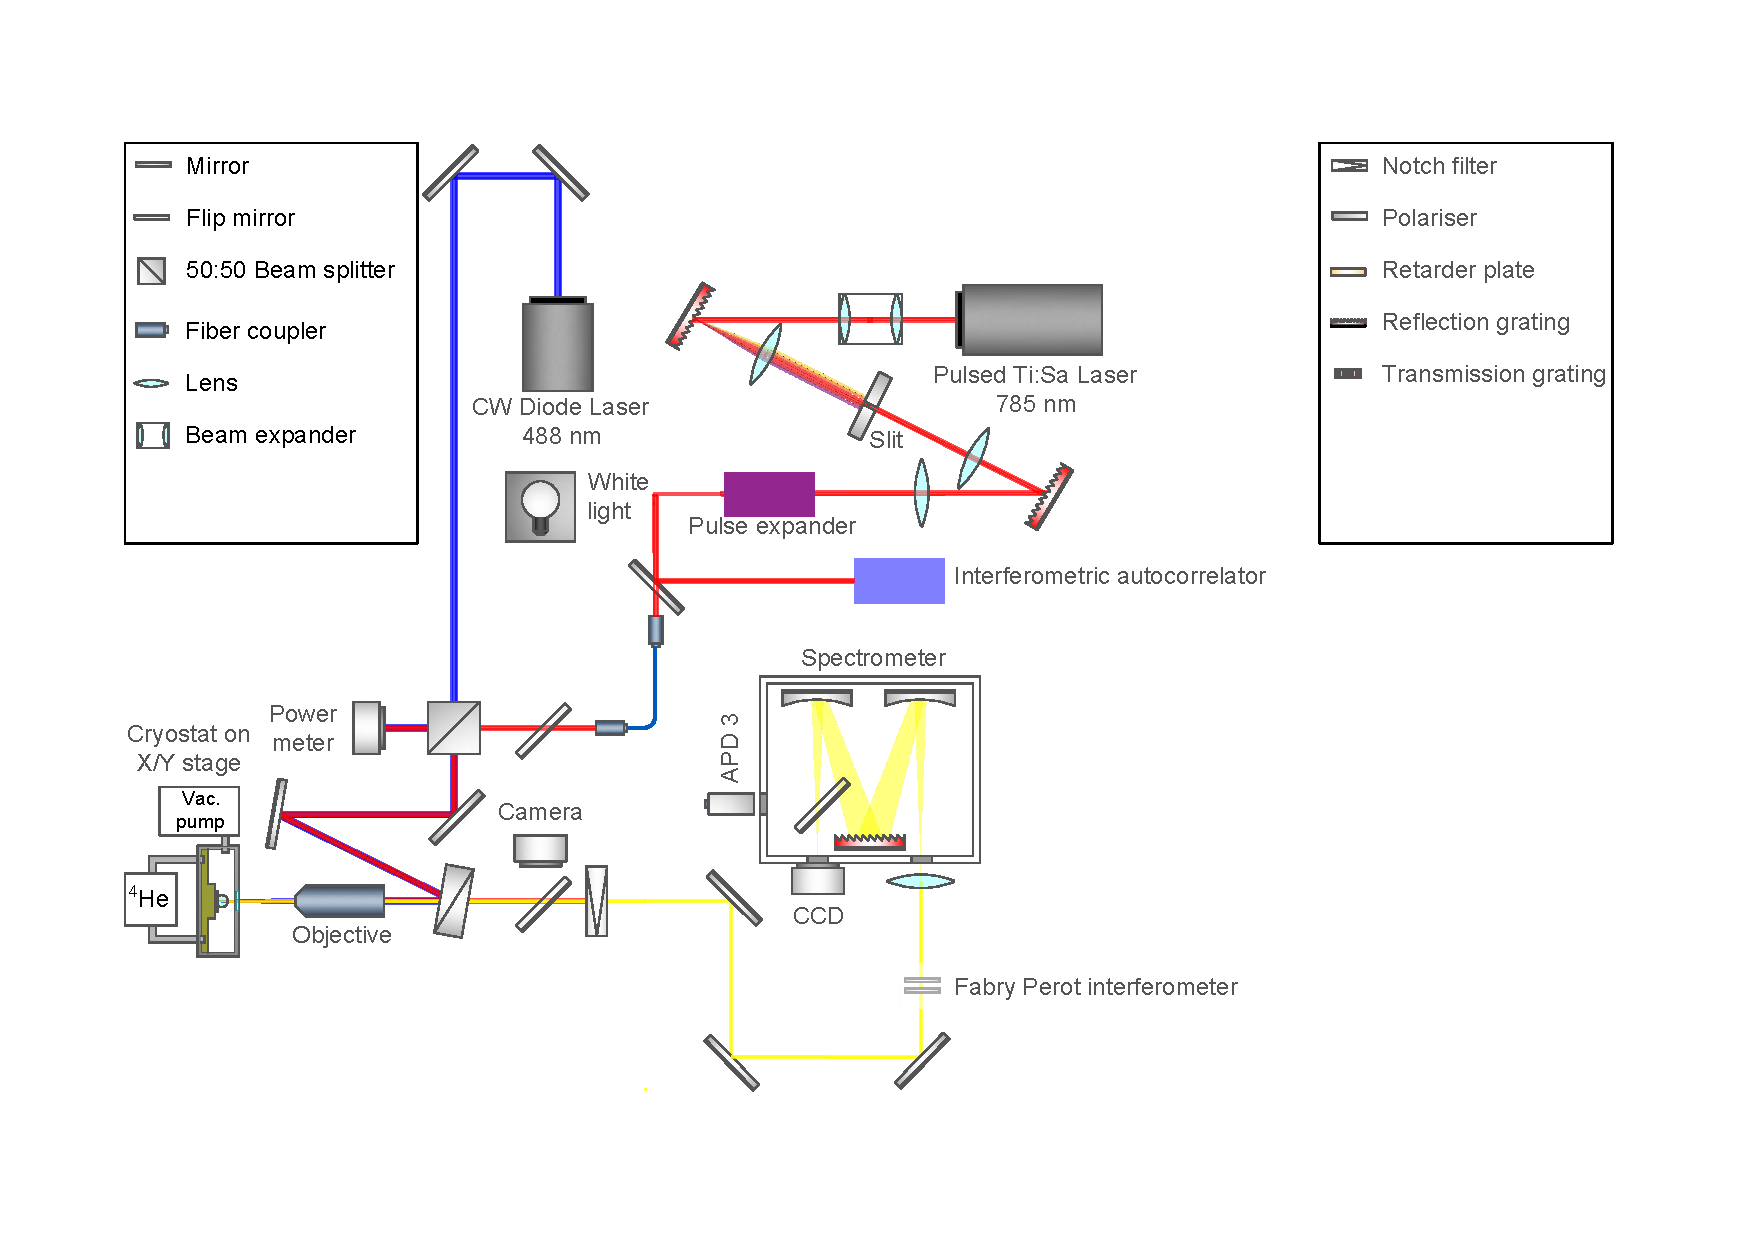
\includegraphics[width=1.1\linewidth]{figures/setup/Setup_flat}
	\caption{Complete experimental setup, which was used in order to quantify the chirp of the Ti:Sa Laser and resolve spectral emission of a quantum dot.}
	\label{fig:setupflat}
\end{figure}
